% TEX program = xelatex
% compile: xelatex -> biber/bibtex -> xelatex -> xelatex
\documentclass[lang=cn,11pt,a4paper]{elegantpaper}

%%% Title
\title{GrabCut 实验报告}
\author{121090003    Bao Jingzhi}
\institute{CUHK(SZ)}
\date{\zhtoday}

%%% main
\usepackage{array}
\usepackage{wrapfig}
\usepackage{listings}
\usepackage{xcolor}
\newcommand{\ccr}[1]{\makecell{{\color{#1}\rule{1cm}{1cm}}}}

\begin{document}

\maketitle

%%% learning objective
\section{预备知识}
\begin{itemize}
    \item[*] 使用 NumPy 和 OpenCV 库处理图像
	\item[*] 图像的对比度估计(直方图归一化,相邻像素值差估计)
    \item[*] 最小费用最大流算法
    \item[*] 使用 \href{https://www.csd.uwo.ca/~yboykov/Papers/iccv01.pdf}{Graph Cut 算法} 进行图像分割
    \item[*] 使用KMeans聚类方法进行数据分析
    \item[*] 使用高斯混合模型提取图像像素值分布的多峰特征并重新建模
	\item[*] 使用 \href{https://cvg.ethz.ch/teaching/cvl/2012/grabcut-siggraph04.pdf}{GrabCut 算法} 进行图像分割
\end{itemize} 

\vspace{10pt}

学习过程整理到了下面的链接中:

\url{https://zmatt.cn/opencv_notebook.html}

\url{https://zmatt.cn/basic_graph_cut_algorithms.html}

\section{开发环境}

\noindent
\textbf{IDE}:Microsoft Visual Studio Code (Universal)\\
\textbf{Python}:3.10.4\\
\textbf{Conda}:4.12.0\\
\textbf{NumPy}:1.21.2\\
\textbf{OpenCV}:4.5.5\\
\textbf{scikit-learn}:1.1.1\\
\textbf{PyMaxflow}:1.2.13

\newpage

\section{Graph Cut}

\subsection{问题描述}
\begin{figure}[ht]
	\centering
	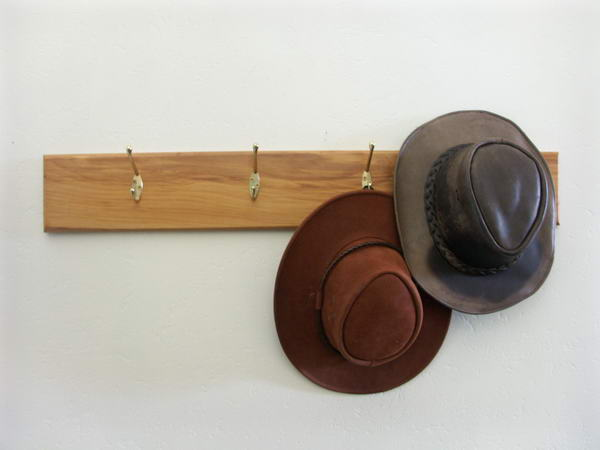
\includegraphics[width=0.5\linewidth]{image/hat.jpg}
	\caption{hat.jpg}
\end{figure}

把图像分成若干个特定的、具有独特性质的区域并提出感兴趣目标(如上图中的帽子),这类问题统称为图像分割问题。

常见的图像分割算法有魔棒(Magic Wand),智能剪刀(Intelligent Scissors),贝叶斯抠图(Bayes matting),水平集(Level sets)等,这些算法各显千秋,而 Graph Cut 算法提出了利用网络最大流对图像建模从而进行图割的思想,往往能取得理想的结果。

\subsection{算法描述}

最小费用最大流算法是解决最优化问题和求最优化方案的常见手段,网络流 24 题集中了许多问题建模方式,在此不做赘述。

\begin{figure}[ht]
    \centering
	\begin{minipage}{0.5\linewidth}
		\centering
		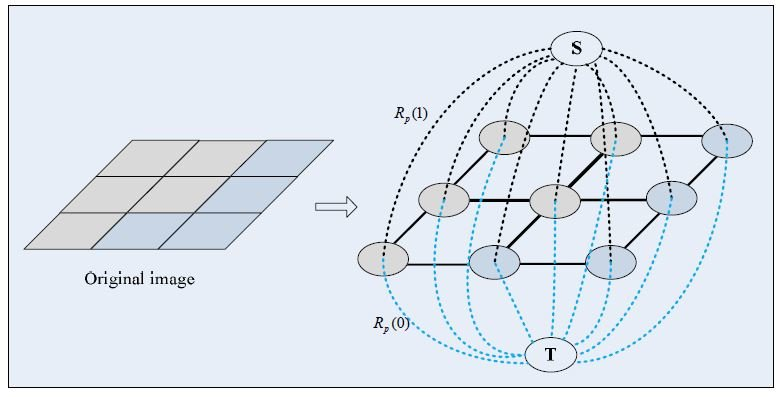
\includegraphics[width=0.9 \linewidth]{image/Illustration-of-s-t-graph-The-image-pixels-correspond-to-the-neighbor-nodes-in-the-model.jpg}
		\caption{Model}
	\end{minipage}%
	\begin{minipage}{0.25\linewidth}
		\centering
		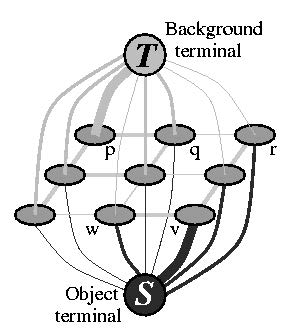
\includegraphics[width=0.8 \linewidth]{image/graph_cut_pic1.jpg}
		\caption{Graph}
	\end{minipage}%
	\begin{minipage}{0.25\linewidth}
		\centering
		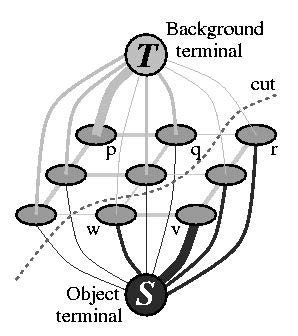
\includegraphics[width=0.8 \linewidth]{image/graph_cut_pic2.jpg}
		\caption{Cut}
	\end{minipage}
\end{figure}

利用网络最大流是 Graph Cut 解决图割问题的核心,其思想是在网络流最小割状态下将前景和背景分配到源点和汇点。算法的难点在于找到一种合理的边权分配方案。

论文给出了一种建模方式,将边权定义为将节点断开的代价,定义图像的总能量为:

\begin{equation}
E(A)=\lambda \cdot R(A)+B(A)
\end{equation}

其中,$A$ 表示输入的图像,$\mathcal{P}$ 表示全体像素,$\mathcal{N}$ 表示邻接像素,$\lambda$ 为加权参数,$R(A)$ 为将像素与源点或汇点断开产生的代价总和,$B(A)$ 为将邻接节点断开产生的代价总和。我们称像素节点与源点和汇点相连的边称为 t-link,邻接像素节点之间的边为 n-link,前景/背景简记为 $\mathcal{O}$, $\mathcal{B}$。

\begin{align}
R(A) & = \sum_{p \in \mathcal{P}} R_{p}\left(A_{p}\right) \\
B(A) & = \sum_{\{p, q\} \in \mathcal{N}} B_{\{p, q\}} \cdot \delta\left(A_{p}, A_{q}\right)
\end{align}

更具体地,所有类型边权的定义如下:

\begin{center}
\begin{tabular}{|c|c|c|}
\hline \textbf{edge} & \textbf{weight (cost)} & \textbf{for} \\
\hline \hline$\{p, q\}$ & $B_{\{p, q\}}$ & $\{p, q\} \in \mathcal{N}$ \\
\hline \multirow{4}{*}{$\{p, S\}$} & $\lambda \cdot R_{p}\text{(``bkg")}$ & $p \in \mathcal{P}, p \notin \mathcal{O} \cup \mathcal{B}$ \\
\cline { 2 - 3 } & $\text{inf}$ & $p \in \mathcal{O}$ \\
\cline { 2 - 3 } & 0 & $p \in \mathcal{B}$ \\
\hline \multirow{4}{*}{$\{p, T\}$} & $\lambda \cdot R_{p}\text{(``obj")}$ & $p \in \mathcal{P}, p \notin \mathcal{O} \cup \mathcal{B}$ \\
\cline { 2 - 3 } & 0 & $p \in \mathcal{O}$ \\
\cline { 2 - 3 } & $\text{inf}$ & $p \in \mathcal{B}$ \\
\hline
\end{tabular}
\end{center}

这里 $R_{p}$ 具体定义为像素 $p$ 在图像的灰度直方图概率分布下概率的对数值的负数, $B_{\{p, q\}}$  需要满足 $p, q$ 与像素值差成反比,于是有:

$$
\begin{array}{l}
R_{p}\left(\text{``obj"}) = -\ln \operatorname{Pr}\left(I_{p} \mid \mathcal{O}\right)\right. \\
R_{p}\left(\text{``bkg"}) = -\ln \operatorname{Pr}\left(I_{p} \mid \mathcal{B}\right) \right. \\
B_{\{p, q\}} \propto \exp \left(-\frac{\left(I_{p}-I_{q}\right)^{2}}{2 \sigma^{2}}\right) \cdot \frac{1}{\operatorname{dist}(p, q)}
\end{array}
$$

\subsection{程序实现}

\subsubsection{选定种子点}

\begin{figure}[ht]
	\centering
	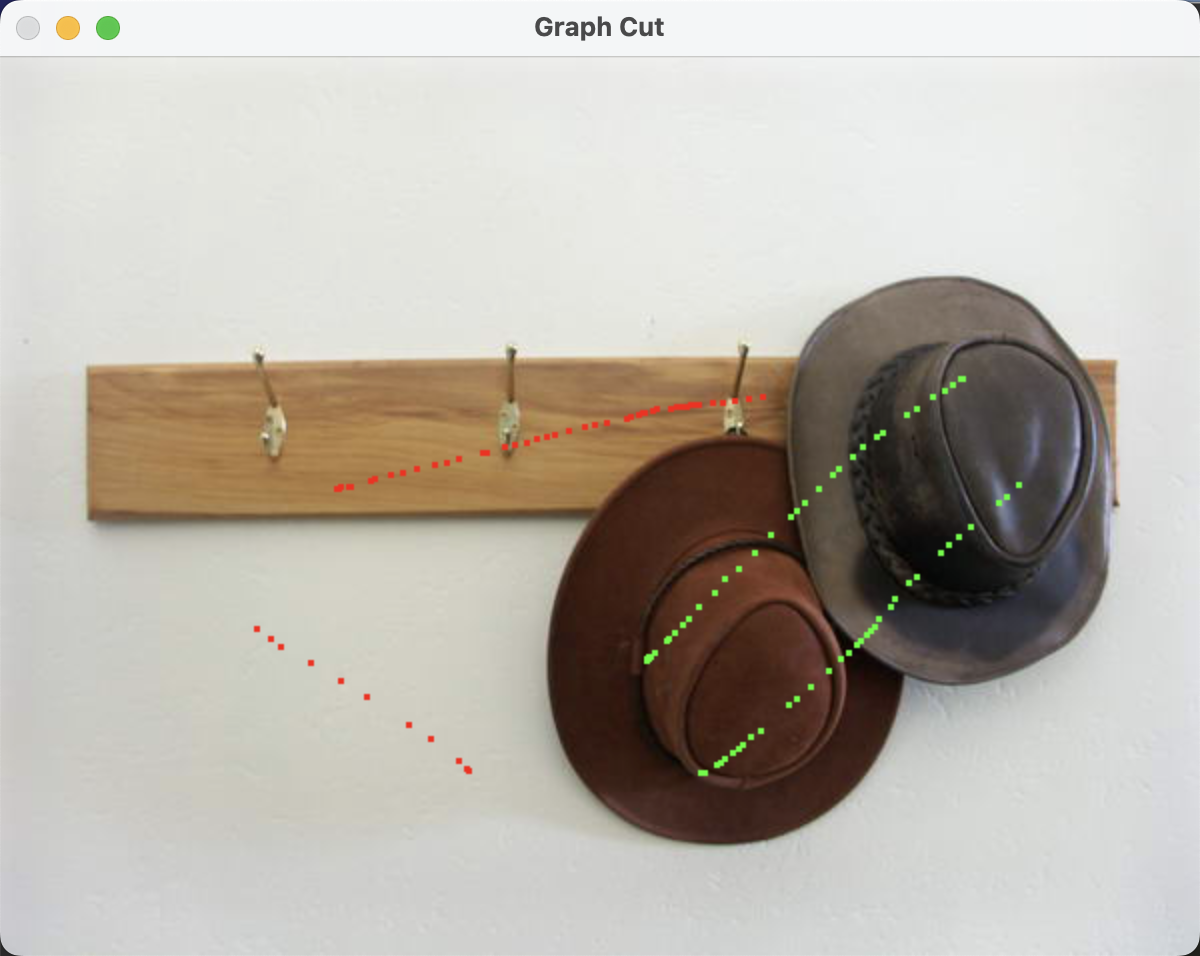
\includegraphics[width=0.5\linewidth]{image/hat_seeds.png}
	\caption{hat\_seeds.png}
\end{figure}

Graph Cut 需要用户选定前景和背景的种子点,图中的绿色点为人为选择的前景样本,红色点为人为选择的背景样本。

\subsubsection{网络流建图}

t-link 的建立部分:

\begin{lstlisting}[language=Python]
def init_grayhist(self):
    self.gray_img = cv.cvtColor(self.img, cv.COLOR_BGR2GRAY)
    cv.normalize(self.gray_img, self.gray_img, 0, 255, cv.NORM_MINMAX, cv.CV_8U)
    self.gray_hist = cv.calcHist([self.gray_img], [0], None, [256], [0, 256])
    # 统计灰度的离散分布信息
    for (y, x), idx in np.ndenumerate(self.graph):
        if idx == 0: self.back_gray_hist[self.gray_img[y, x]] += 1
        elif idx == 1: self.fore_gray_hist[self.gray_img[y, x]] += 1
            
def calc_gray(self, y, x):
    num = self.gray_img[y, x]
    p1, p2 = self.back_gray_hist[num], self.fore_gray_hist[num]
    return -np.log(p1 / (p1+p2)), -np.log(p2 / (p1+p2)) # 计算 t-link 的边权
\end{lstlisting}

n-link 的建立部分:

\begin{lstlisting}[language=Python]
def n_link(self):
    for (y, x), idx in np.ndenumerate(self.graph):
        k = y * self.w + x
        if x != self.w-1:
            w = 1. / (1. + np.sum(np.power(self.img[y,x+1]-self.img[y, x],2) / 2))
            self.add_edge(k, k+1, w, w)
        if y != self.h-1:
            w = 1. / (1. + np.sum(np.power(self.img[y+1,x]-self.img[y, x],2) / 2))
            self.add_edge(k+self.w, k, w, w)
\end{lstlisting}

\subsection{成果展示}

\begin{figure}[ht]
	\centering
	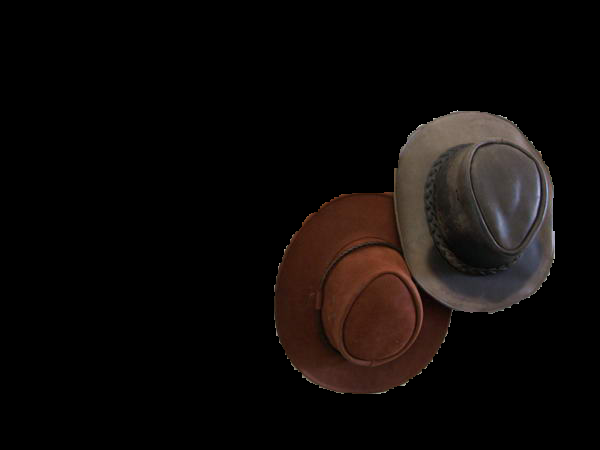
\includegraphics[width=0.45\linewidth]{image/hat_result.png}
	\caption{hat\_result.png}
\end{figure}

\section{GrabCut}

\subsection{算法描述}

GrabCut 算法是 Graph Cut 算法的改进,主要体现在两个方面:(1)  引入了更多的参数以利用更丰富的图像信息;(2)  从一次性求解改为了不断迭代更新图像分割的解。

GrabCut 将全体像素分为四类:前景样本,背景样本,可能前景区域,可能背景区域。前景样本和背景样本与 Graph Cut 算法相同,除此之外,用户需要额外框定可能前景区域,剩余的像素将初始化为可能背景区域。

论文提出了要让 t-link 的权值体现前景/背景的色彩特征,于是将灰度直方图概率替换为高斯混合模型(GMM)。对于图像中的两类模糊区域内分别用 KMeans 聚类方法将像素分为 $K$ 类,从而得到高斯混合模型中的峰值特征。为还原图像RGB色彩的高斯混合模型,只需要将这 $K$ 个聚类根据其大小分配权值。最终概率模型为这 $K$ 个概率的加权和,即

$$
\begin{array}{l}
\operatorname{Pr}(I_{p}) =  \sum\limits_{i=1}^{k} w_i \cdot \operatorname{Pr}_{i}(I_{p})
\end{array}
$$

注意在RGB色彩空间中像素 $X^{3\times1}$ 在高斯分布中的概率为:

$$
\begin{array}{l}
p(X)=\cfrac{1}{(2 \pi)^{\frac{d}{2}}|\Sigma|^{\frac{1}{2}}} \exp \left\{-\frac{1}{2}(X-\mu)^{T} \Sigma^{-1}(X-\mu)\right\}
\end{array}
$$

论文也提出了改进 n-link 权值的方法,相较于 Graph Cut,边权根据图像整体对比度进行调整,以避免图像本身的对比度过强造成过度分割。

\begin{equation}
    V(\underline{\alpha}, \mathbf{z})=\gamma \sum_{(m, n) \in \mathbf{C}}\left[\alpha_{n} \neq \alpha_{m}\right] \exp -\beta\left\|z_{m}-z_{n}\right\|^{2}
\end{equation}

其中 $\gamma$ 为权衡 t-link 和 n-link 的参数常量(论文建议设置为 50 ),$\beta$ 是体现图像对比度的参数,计算公式为:

\begin{equation}
    \beta=\left(2\left\langle\left(z_{m}-z_{n}\right)^{2}\right\rangle\right)^{-1}
\end{equation}

至此,网络流建模已有据可循。最终的算法流程为:(1) 根据用户选择初始化前景和背景的 GMM,得到像素的初始区域(前景/背景)分配;(2) 对全体像素分配其所在区域内的 GMM 聚类分量 $k$;(3) 学习 GMM 的模型参数 $\mu^{3\times1}$, $\Sigma^{3\times3}$,$w_i$;(4) 根据 GMM 模型建图;(5) 求网络流的最小割,得到像素的区域(前景/背景)分配,再返回 (2)。

\subsection{程序实现}

\subsubsection{高斯混合模型}

\begin{lstlisting}[language=Python]
def initGMM(self, rect, iternum = 200):
    # 模型初始化
    KMeans_model_fore = KMeans(n_clusters = k, max_iter = iternum)
    fore_res = KMeans_model_fore.fit(self.foreSamples)
    KMeans_model_back = KMeans(n_clusters = k, max_iter = iternum)
    back_res = KMeans_model_back.fit(self.backSamples)
    # 在 k 聚类中分别添加对应的样本
    for i in range(len(self.foreSamples)):
        self.foreGMM.addSample(fore_res.labels_[i], self.foreSamples[i])
    for i in range(len(self.backSamples)):
        self.backGMM.addSample(back_res.labels_[i], self.backSamples[i])

def Learning(self):
    # 高斯混合模型参数学习
    variance = 0.01
    for ci in range(k):
        n = self.count[ci]
        if n == 0:
            self.weight[ci] = 0
        else:
            self.weight[ci] = n / self.total_count
            self.mean[ci] = self.sum[ci] / n
            mean_tmp = self.mean[ci].reshape(-1, 1)
            self.cov[ci] = self.prod[ci]/n-np.dot(mean_tmp,np.transpose(mean_tmp))
            self.cov_det[ci] = np.linalg.det(self.cov[ci])
            # 添加白噪声防止矩阵退化
            while self.cov_det[ci] <= 0:
                self.cov[ci] += np.diag([variance, variance, variance])
                self.cov_det[ci] = np.linalg.det(self.cov[ci])
            self.cov_inv[ci] = np.linalg.inv(self.cov[ci])
\end{lstlisting}

\subsubsection{分配像素的GMM分量}

\begin{lstlisting}[language=Python]
def Pr(self, ci, color):
    diff = np.asarray([color - self.mean[ci]])
    mult = np.dot(diff, np.dot(self.cov_inv[ci], np.transpose(diff)))[0][0]
    return np.exp(-0.5 * mult) / np.sqrt(self.cov_det[ci]) / np.sqrt(2 * np.pi)

def whichComponent(self, color):
    # 返回 k 个聚类中的概率最大项
    prob = np.asarray([self.Pr(ci, color) for ci in range(k)])
    return prob.argmax(0)
\end{lstlisting}

\subsubsection{网络流建图}

这一部分与 Graph Cut 的建图部分相同,仅更新了公式,故不再赘述。

\subsection{成果展示}

左、中、右分别为原图、交互图、分割结果。原图来源网络。

\begin{figure}[ht]
	\centering
	\begin{minipage}{0.3\linewidth}
		\centering
		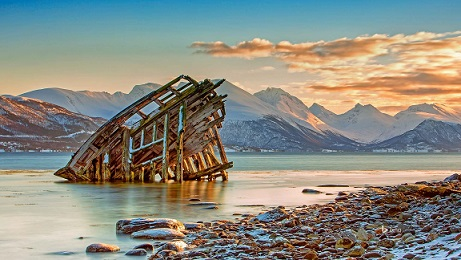
\includegraphics[width=0.95\linewidth]{image/boat.jpg}
	\end{minipage}
	\begin{minipage}{0.3\linewidth}
		\centering
		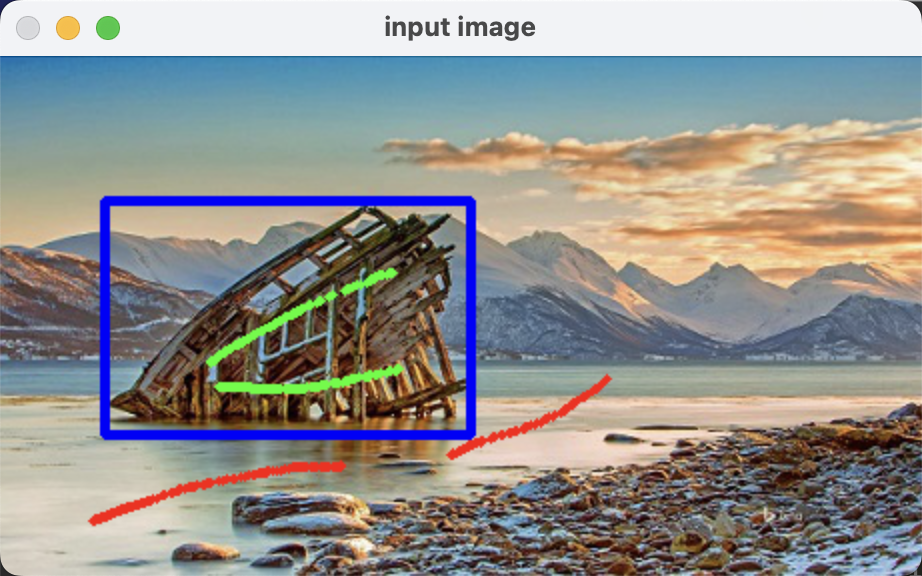
\includegraphics[width=0.95\linewidth]{image/boat_graffiti.png}
	\end{minipage}
	\begin{minipage}{0.3\linewidth}
		\centering
		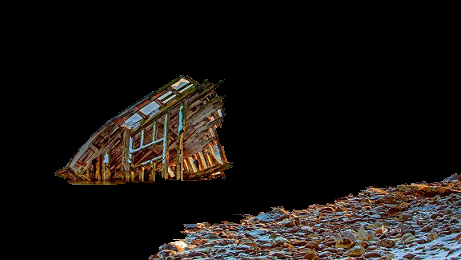
\includegraphics[width=0.95\linewidth]{image/result_boat_.png}
	\end{minipage}%
	%让图片换行,
	
	\begin{minipage}{0.3\linewidth}
		\centering
		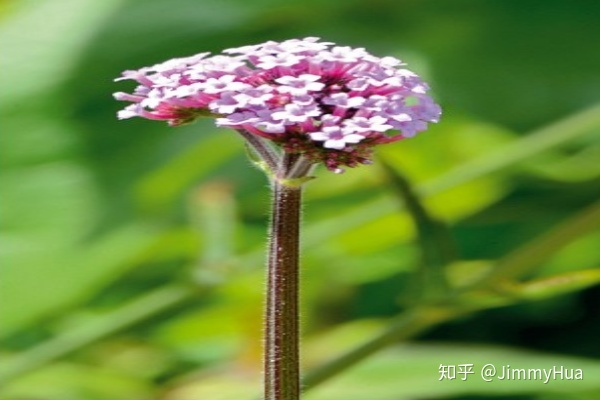
\includegraphics[width=0.95\linewidth]{image/flower.jpeg}
	\end{minipage}
	\begin{minipage}{0.3\linewidth}
		\centering
		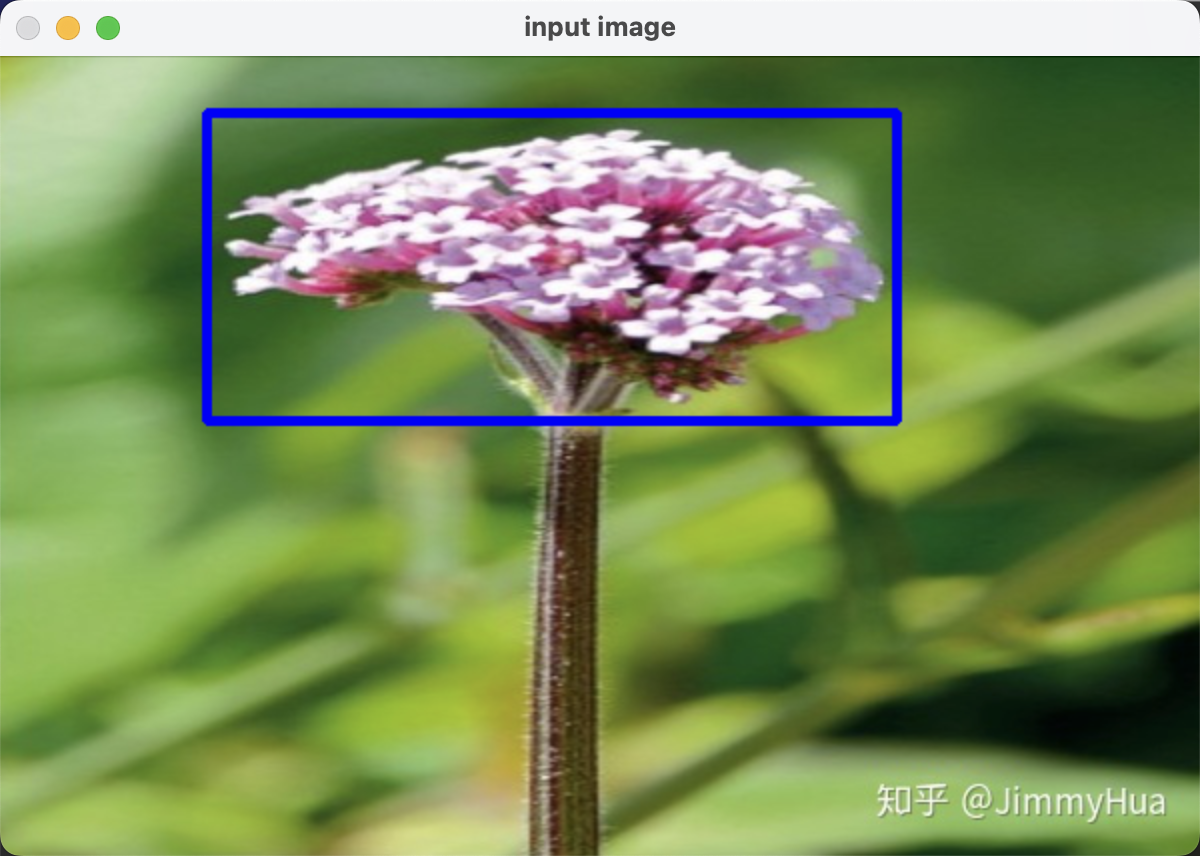
\includegraphics[width=0.9\linewidth]{image/flower_graffiti.png}
	\end{minipage}
	\begin{minipage}{0.3\linewidth}
		\centering
		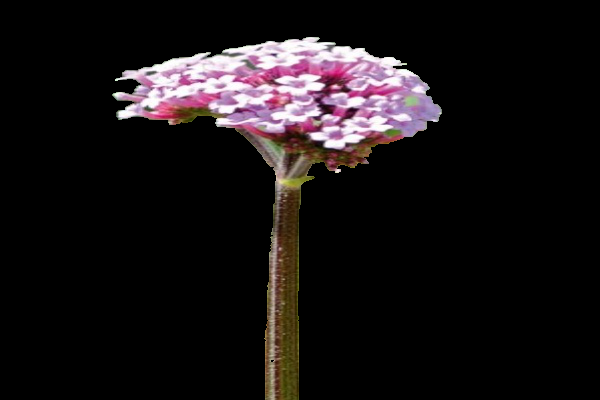
\includegraphics[width=0.9\linewidth]{image/result_flower_.png}
	\end{minipage}%
	%
	
	\begin{minipage}{0.3\linewidth}
		\centering
		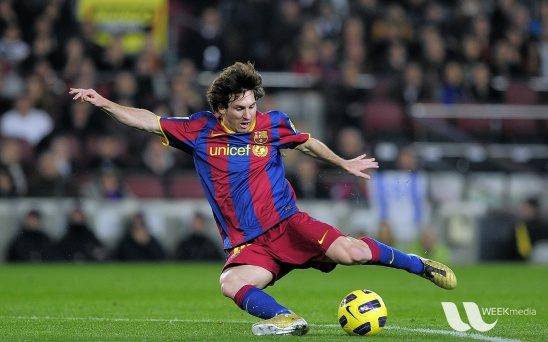
\includegraphics[width=0.95\linewidth]{image/messi.jpg}
	\end{minipage}
	\begin{minipage}{0.3\linewidth}
		\centering
		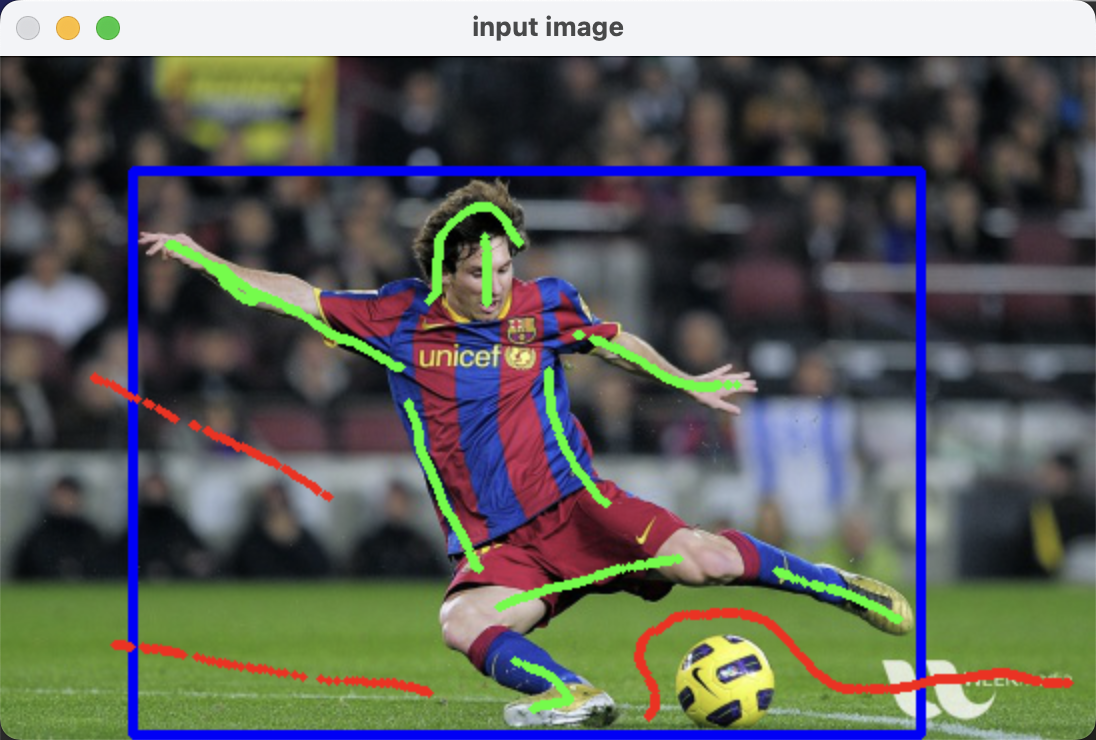
\includegraphics[width=0.9\linewidth]{image/messi_graffiti.png}
	\end{minipage}
	\begin{minipage}{0.3\linewidth}
		\centering
		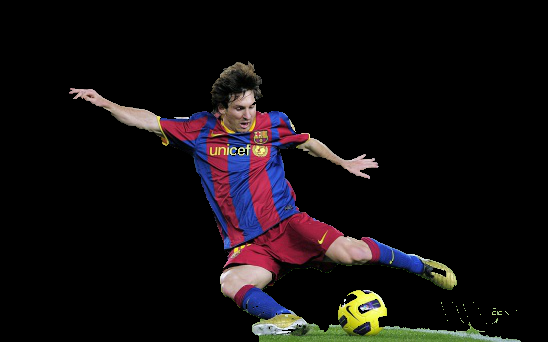
\includegraphics[width=0.9\linewidth]{image/result_messi.png}
	\end{minipage}
\end{figure}

细节展示:

\begin{figure}[ht]
	\centering
	\begin{minipage}{0.3\linewidth}
		\centering
		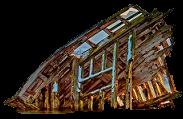
\includegraphics[width=0.98\linewidth]{image/result_boat_details.png}
	\end{minipage}
	\begin{minipage}{0.3\linewidth}
		\centering
		
\includegraphics[width=0.98\linewidth]{image/result_flower_details.png}
	\end{minipage}
	\begin{minipage}{0.3\linewidth}
		\centering
		
\includegraphics[width=0.98\linewidth]{image/result_messi_details.png}
	\end{minipage}
\end{figure}

\section{其他图像分割算法概述}

这一部分是对论文中所提到的图像分割算法的概述。

\subsection{魔棒 Magic Wand}

原理:从图像中指定的种子点(seed point)开始扩充(宽度优先搜索BFS),将相邻像素值的差异值超过包容程度(tolerance level)的区域记为边界,最终获得有闭合边界的区域。这种算法应用在 Adobe Photoshop 中的魔棒工具。

缺点:设置不同的 tolerance level 会得到完全不同的区域且交互信息过于简单,仅有图像中一个种子点(seed point),得到的分割结果常常不理想。

\subsection{智能剪刀 Intelligent Scissors}

原理:跟踪用户鼠标移动,以鼠标位置为参考点实时查找物体的强边界特征并进行吸附(cool down)。这里图像边界提取的依据为最小化图像区域代价(Image  Local Cost),这个代价由六项特征值组成,分别为拉普拉斯交叉零点(Laplacian zero-crossing),梯度值(Gradient magnitude),梯度方向值(Gradient direction),边界像素灰度值(Edge pixel value),边界像素灰度值(Inside pixel value),外部像素灰度值(Outside pixel value)。即利用代价函数
\begin{equation}
    \begin{aligned}
        &l(p, q)=\omega_{Z} \cdot f_{Z}(q) +\omega_{D} \cdot f_{D}(p, q) +\omega_{G} \cdot f_{G}(q) \ \text{or} \\
        &l(p, q)=\omega_{Z} \cdot f_{Z}(q)+\omega_{G} \cdot f_{G}(q)+\omega_{D} \cdot f_{D}(p, q)+\omega_{P} \cdot f_{P}(q)+\omega_{I} \cdot f_{I}(q)+\omega_{O} \cdot f_{O}(q)
    \end{aligned}
\end{equation}
在有限区域内进行动态规划解代价最小点,从而得到理想边界点。这种算法应用在 Adobe Photoshop 中的磁性套索工具。(参考论文:\href{https://dl.acm.org/doi/pdf/10.1145/218380.218442}{Intelligent Scissors for Image Composition}, \href{https://www.sciencedirect.com/science/article/pii/S1077316998904804}{Interactive segmentation with Intelligent Scissors})

缺点:对纹理信息很敏感,在纹理非常明显或无纹理的图片表现很差,需要不断人为加入 seeds 纠正路径。

\subsection{贝叶斯抠图 Bayes matting}

原理:此分割算法提出了一个新的概念 trimap,记录用户指定的前景区、背景区、模糊区,将问题转化为解方程 $C=\alpha F+(1-\alpha) B$ ,其中 $C$ 为给定图像, $F$ 为待求解的前景区,$B$ 为待求解的背景区。求出这个方程的解十分困难,论文作者简化了局部方程和参数,将问题转化为了求解似然方程:
\begin{equation}
    \underset{a, F, B}{\arg \max } L(C \mid \alpha, F, B)+L(\alpha)+L(F)+L(B)
\end{equation}
其中 $L(C \mid \alpha, F, B)$ 以图像像素值高斯分布下的方差作为衡量依据, $L(F)$ 和 $L(B)$ 以高斯混合模型下采样点到聚类中心的马氏距离(Mahalanobis distance)定义代价。方程的求解需要对上述的似然函数求导,得到方程组。为启动迭代算法,作者初始化 $\alpha$ 值为 trimap 区域的前景区 $\alpha$ 的均值,再不断迭代更新 $\alpha$, $L$, $B$, 得到最终的解。对未知像素(trimap 中的模糊区)分配区域时,论文采用解边缘局部,以滑动窗口的思想不断向未知像素块内部求解,从而提高分配的准确性。此方法中对似然方程的求解运算较为复杂,但得到的结果较为理想。(参考论文:\href{https://grail.cs.washington.edu/projects/digital-matting/papers/cvpr2001.pdf}{A Bayesian Approach to Digital Matting})

缺点:作者为求解实际方程进行了诸多假设,理论上不具有普适性。图像求解速度慢,方程复杂。当目标边缘局部色彩和背景相似时,这种方法无法对前景和背景进行准确的归类。

\subsection{Knockout 2}

Knockout 2 是 Adobe Photoshop 的一个插件,操作过程和成品效果与 Bayes matting 类似,尚未公开相关论文和代码,暂且不作分析。

\subsection{水平集 Level sets}

水平集(Level sets)算法也称Snake算法,是一类解偏微分方程的思想,在其之上定义能量泛函后可以将其转化为最优化问题。在图像中定义合适的代价函数可以进行图像分割。这一部分涉及的数学知识较深,目前仅了解大致思想。

原理:本质上是利用更高维度的函数 $f(x,y)$ 与 $z=0$ 的平面的交线来体现目标物体的轮廓线,根据曲线的偏微分方程进行函数迭代。为实现图像分割,需要定义能量泛函对偏微分方程中的参数施加限制。定义合适的能量泛函后得到的曲线 $f(x,y)=0$ 便是目标物体的轮廓线。 (参考论文:\href{https://link.springer.com/article/10.1023/A:1007979827043}{Geodesic active contours})

缺点:很难找到具有普适性的代价函数。最终图像的结果对初始化过程中的的区域选择较为敏感。

\section{总结}

图像分割问题存在许多解决方案,不同的方案有不同的切入点,得到的结果也不尽相同。尽管如此,这些方法在对图像建模的思想也都殊途同归。例如 魔棒(Magic Wand) 算法的种子点思想,在 Graph Cut 和 水平集(Level sets) 中也有直接的应用,智能剪刀(Intelligent Scissor) 的修正思想(cool down)也与设置种子点本质上相同。贝叶斯抠图(Bayes matting)和 Grab Cut 都有迭代更新求解的思想,并且都运用了统计学中的概念对像素信息进行聚类分析,得到概率模型,从而定义代价函数。

图像分割问题的难点在于定义合适的代价函数,从而通过图像的像素值信息,准确地量化前景和背景的差异。

上述算法往往都能取得良好的分割结果,但各有其局限性,具体体现在求解时间、图像特征干扰(如曝光、生物特征)、模型假设等方面。这些算法与机器学习方法相结合,可能能避免一部分问题。

此外,这篇论文的一位作者 Vladimir Kolmogorov 和 Graph Cut 论文的一位 Yuri Boykov 曾发表过一篇关于网络流最小割的论文 \href{https://ieeexplore.ieee.org/document/1316848}{An Experimental Comparison of Min-Cut/Max-Flow Algorithms for Energy Minimization in Vision}. 在求解网络流最小割上要比传统的 Dinic 算法,ISAP 算法以及更优秀的 Push-Relabel 预流推进算法, HLPP 算法更适合解决这类问题,从而很好地优化了最小割问题的求解时间。

\end{document}